\documentclass[twoside]{book}

%---------------------------------------------------------------
%   PACKAGES
%---------------------------------------------------------------
\usepackage{graphicx} % Required for inserting images
\usepackage{xcolor}
\usepackage{acronym}
\usepackage{tabularx}
\usepackage{longtable}
\usepackage{colortbl}
\usepackage{float}
\usepackage{listings}
\usepackage{rotating}
\usepackage{hyperref}

%---------------------------------------------------------------
%   ALLOY CONFIG
%---------------------------------------------------------------
\lstdefinelanguage{alloy}{
    morekeywords={
        module, open, as,
        private, abstract, sig, extends, in,
        lone, some, one, disj,
        fact, pred, fun, assert,
        run, check,
        for, but, exactly,
        this, not, implies, else, let,
        not, no, set, all, sum,
        iff, or, Int, and,
        none, univ, iden
    },
    sensitive=true,
    morecomment=[l]{//},
    morecomment=[l]{--},
    morecomment=[s]{/*}{*/},
    morestring=[b]{"},
%literate={->}{$\rightarrow$}1
% replacing characters can cause problems when copying from PDF to editor
}[keywords,comments,strings]

\definecolor{dkgreen}{rgb}{0,0.6,0}
\definecolor{gray}{rgb}{0.5,0.5,0.5}
\definecolor{mauve}{rgb}{0.58,0,0.82}


\lstset{frame=tb,
    language=alloy,
    aboveskip=3mm,
    belowskip=3mm,
    showstringspaces=false,
    columns=flexible,
    basicstyle={\small\ttfamily},
    numbers=none,
    numberstyle=\tiny\color{gray},
    keywordstyle=\bf\color{blue},
    commentstyle=\it\color{dkgreen},
    stringstyle=\color{mauve},
    breaklines=true,
    breakatwhitespace=true,
    tabsize=3
}

%---------------------------------------------------------------
%   NEW COMMANDS
%---------------------------------------------------------------

\newcommand{\newtext}[1]{\textcolor{blue}{#1}}
\newcommand{\myworries}[1]{\textcolor{red}{#1}}

%---------------------------------------------------------------
%   ACRONYMS
%---------------------------------------------------------------


\acrodef{CKB}[CKB]{CodeKataBattle}
\acrodef{CK}[CK]{CodeKata}


%---------------------------------------------------------------
%   DOCUMENT
%---------------------------------------------------------------

\begin{document}


\title{RASD}
\author{Federico Valentino, Nicola Zarbo }
\date{October 2023}


\maketitle
\newpage
\setcounter{page}{1}

\tableofcontents % Table of contents
\cleardoublepage

\chapter{Introduction}
\section{Purpose}
\ac{CKB} is a new platform that helps students improve their software development skills by training with peers on code katas . Educators use the platform to challenge students by creating code kata battles in which teams of students can compete against each other, thus proving (and improving) their skills.\newline
A code kata battle is essentially a programming exercise in a programming language of choice (e.g., Java, Python). The exercise includes a brief textual description and a software project with build automation scripts (e.g., a Gradle project in case of Java sources) that contains a set of test cases that the program must pass, but without the program implementation. Students are asked to complete the project with their code. In particular, groups of students participating in a battle are expected to follow a test-first approach and develop a solution that passes the required tests. Groups deliver their solution to the platform (by the end of the battle). At the end of the battle, the platform assigns scores to groups to create a competition rank.
\subsection{Goals}
The \ac{CKB} system is thought, designed and proposed to two types of users: Students and Educators.\newline
The firsts, will be able to join the platform to test their coding skills in Tournaments, a series of code battles, where students will be able to participate in groups.\newline
Educators instead will be able to create and manage tournaments and decide whether or not a manual score in a battle is needed or not.\newline
Below the list of goals of the \ac{CKB} platform.\newline

\begin{center}
    \begin{longtable}{ |l|p{0.9\linewidth}| }
        \hline
        \textbf{ID} & \textbf{Description}\\
        \hline
        G1 & An Educator can manage a tournament. \\
        \hline
        G2 & An educator can create battles inside of a tournament in which he is involved. \\
        \hline
        G3 & Students can participate in tournaments created by an educator\\
        \hline
        G4 & Students can participate and compete in battles created by an educator, alone or in groups. \\
        \hline
        G5 & Students are scored based on their performance in battles. \\
        \hline
        G6 & The platform allows students and educators to compare the performance of students. \\
        \hline
        \caption{The goals.}
    \end{longtable}
\end{center}


\section{Scope}
\subsection{World phenomena}
\begin{center}
    \begin{longtable}{ |l|p{0.9\linewidth}| }
        \hline
        \textbf{ID} & \textbf{Description}\\
        \hline
        W1 & An educator wants to create a tournament to evaluate students performance. \\
        \hline
        W2 & Students fork the created repository for a battle on Github. \\
        \hline
        W3 & An educator creates the battle assignment. \\
        \hline
        W4 & Students write source code for the code kata battle. \\
        \hline
        W5 & Students create commits on Github. \\
        \hline
        W6 & Students decide to join a battle. \\
        \hline
        W7 & Students create groups for battles. \\
        \hline
        W8 & Students setup an automated workflow for the forked repository on Github. \\
        \hline
        W9 & Students decide to join a tournament. \\
        \hline
        W10 & Educator decides to close tournament. \\
        \hline
        \caption{World Phenomenas.}
    \end{longtable}
\end{center}
\subsection{Shared phenomena}

\begin{center}
    \begin{longtable}{ |l|p{0.5\linewidth}|l|l| }
        \hline
        \textbf{ID} & \textbf{Description} & \textbf{Controller} & \textbf{Observer}\\
        \hline
        SP1 & An educator fills out a tournament creation form. & Educator & \ac{CKB}\\
        \hline
        SP2 & An educator uploads the details of a code kata battle(the assignment, the rules, the tests). & Educator & \ac{CKB} \\
        \hline
        SP3 & A group(maybe singleton) joins a battle respecting the rules regarding the min and max group size. & Student & \ac{CKB}\\
        \hline
        SP4 & An educator logs into the platform. & Educator & \ac{CKB} \\
        \hline
        SP5 & A student logs into the platform. & Student & \ac{CKB}\\
        \hline
        SP6 &  The system requires additional manual evalution by an educator for a battle(if required by the rules). & Educator & \ac{CKB}\\
        \hline
        SP7 & The educator inserts an additional manual score for a battle. & Educator & \ac{CKB}\\
        \hline
        SP8 & A student invites other students to a group to participate to a battle. & Student & \ac{CKB}\\
        \hline
        SP9 & Github on commit notifies the code kata platform. & GitHub & \ac{CKB}\\
        \hline
        SP10 & An educator registers an account on the platform. & Educator & \ac{CKB}\\
        \hline
        SP11 & A student registers an account on the platform. & Student & \ac{CKB}\\
        \hline
        SP12 & A student subscribes to a tournament. & Student & \ac{CKB}\\
        \hline
        SP13 & Students and educators look at the rank for a battle they are involved in. & User & \ac{CKB} \\
        \hline
        SP14 & Students and educator look at the rank for a tournament. & User & \ac{CKB}\\
        \hline
        SP15 & Educator closes tournament. & Educator & \ac{CKB}\\
        \hline
        SP16 & User looks at list of available tournament. & User & \ac{CKB}\\
        \hline
        SP17 &  A student accepts and invitet o a group to partecipate to a battle. & Student & \ac{CKB}\\
        \hline
        SP18 & The platform notifies all students when a tournament is created. & \ac{CKB} & Student\\
        \hline
        SP19 & The platfotm notifies all students subscribed to a tournament of new upcoming battles.& \ac{CKB} & Student\\
        \hline
        SP20 & The platform notifies the final score to all students subscribed to a battle, when that battle ends.& \ac{CKB} & Student\\
        \hline
        SP21 & When the platform is notifies about a commit, it pulls from the committed repository to start the mandatory analysis.& \ac{CKB} & Github\\
        \hline
        SP22 & The platform creates the github repository for a battle.& \ac{CKB} & Github\\
        \hline
        SP23 & The platform sends links to the created repository for the battle to all students who are subscribed to the battle.& \ac{CKB} & Student\\
        \hline
        \caption{Shared Phenomenas.}
    \end{longtable}
\end{center}

\section{Definitions, Acronyms, Abbreviations}

\begin{table}[H]
    \begin{center}
        \begin{tabular}{|l|l|}
            \hline
            \textbf{Acronym} & \textbf{Definition}\\
            \hline
            CKB & CodeKataBattle\\
            \hline
            CK & Code Kata\\
            \hline
        \end{tabular}
        \caption{Acronyms used in the document}
    \end{center}
\end{table}

\section{Document Structure}
The document is divided in six sections. \newline
The first section introduces the goals of the project and shared phenomena with also a list of definitions useful to understand the problem.\newline
The second section provides a more accurate description of the problem, describing the details of domain and scenarios.\newline
The third section focuses on specific requirements and provides an analysis on interface requirements, functional requirements and so on.\newline
The fourth section provides a formal analysis using Alloy, crucial to prove the correctness of the model described.\newline
The fifth one reports the effort spent by each group member in the redaction of this document and the last section is simply a list of bibliography references.
\newpage

\chapter{Overall description}
\section{Product perspective}
\subsection{Class Diagrams}
The diagram below represents and describes the classes involved in the system, their functionalities and how they interact.

\begin{figure}[ht]
    \centering
    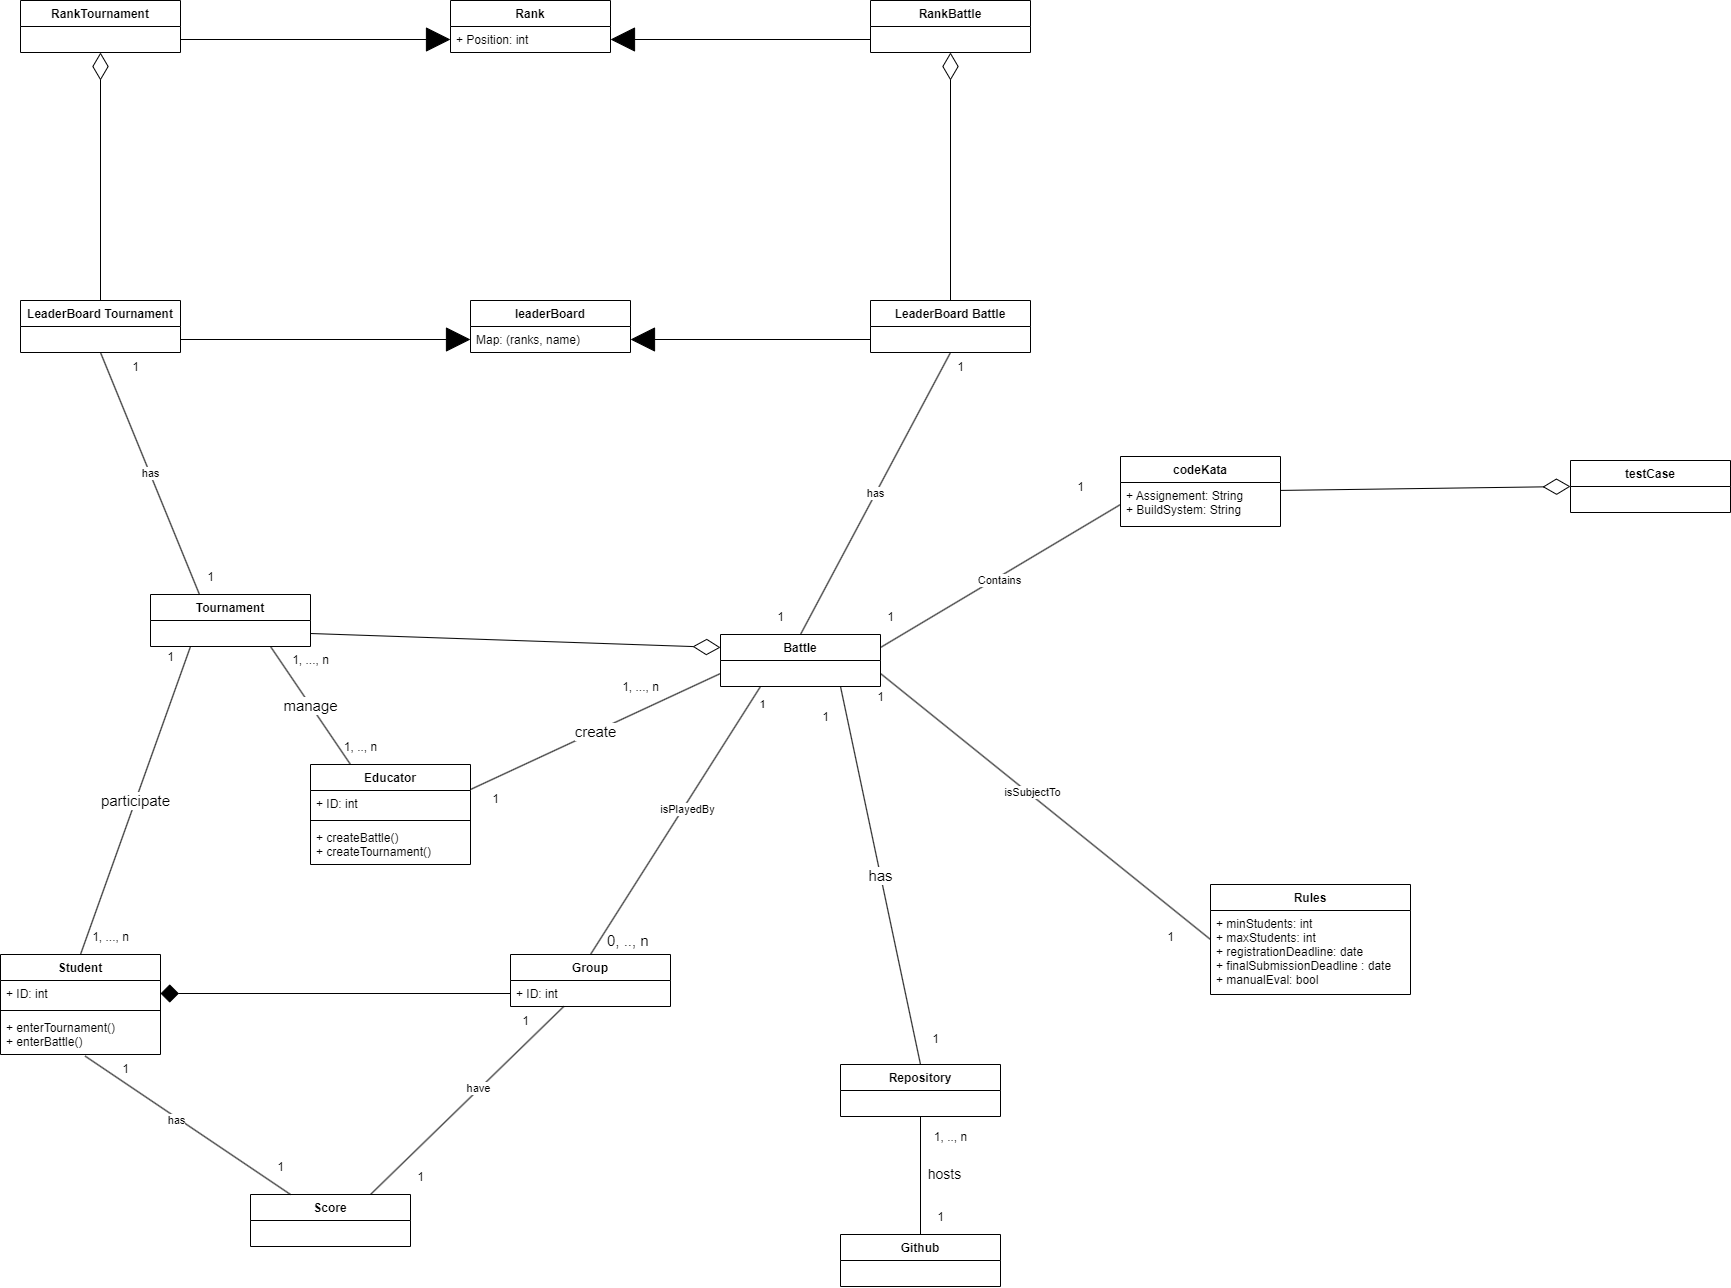
\includegraphics[width=1\linewidth]{misc//Images/classDiagram.png}
    \caption{Class Diagram}
    \label{fig:enter-label}
\end{figure}



\subsection{Scenarios}
\begin{enumerate}
    \item \textbf{User signs into platform}\newline
    Professor Layton wants to evaluate the performance of his programming students but he has no easy way to do so. Fortunately he knows about \ac{CKB} that can allow him to write a few coding challenges and automatically score his students submissions. He reaches the platform and is presented with a Sign In page where he has to full fill his details and set his profile to educator.\newline Luke is a student of Professor Layton and when he heard that the professor is using \ac{CKB} he immediately reached it and signed up by full filling his details and setting his profile to student.
    
    \item \textbf{User logs into platform}\newline
    A student that want to access the functionalities of the platform can log in , an educator does the same.
    
    
    \item \textbf{Educator creates tournament}\newline
    Professor Layton, now signed into \ac{CKB}, can create a new tournament and add collaborators to it. Once the tournament has been created every user subscribed to the \ac{CKB} platform is notified and can enter it.
    
    \item \textbf{Educator creates battle}\newline
    An educator wants to add another battle in the context of a tournament he is partecipating in. 
    He starts by creating a \ac{CK} assignment (containing description, software project, test cases and build automation scripts) and ultimately creates the battle using the \ac{CKB} platform.  
    On the \ac{CKB} platform the educator then uploads the \ac{CK} assignment and sets:
    \begin{itemize}
        \item minimum and maximum number of students per group,
        \item set a registration deadline,
        \item set a final submission deadline,
        \item set additional configurations for optional manual scoring 
    \end{itemize}
    
    Once the battle in is created all the students subscribed to the tournament of said battle receive a notification of its creation.
    
    \item \textbf{Student subscribes to a tournament}\newline
    Once a student is logged into the website he is presented with a list of available tournaments he can join. By clicking on one of them the tournament description will be available for him to read and if he wants he can click on join to take part in that tournament.
    
    \item \textbf{Student joins a team for a battle}\newline
    The students are notified of a new battle in the context of a tournament.
    A student that decides to join the battle may be asked to join as a group (in case the battle rules ask for it ), and so he invites other students using the \ac{CKB} platform to create a group that respects the group dimension rule.  
    Once every student accepts the new group joins the battle.   
    
    Once the subscription deadline expires the \ac{CKB} platform creates a GitHub repository containing the \ac{CK} and sends every student a link for it.  
    At this point for every group the students fork the repository and set up the automated workflow with Github Actions.
    At this point the group is ready to start working on the \ac{CK}.
    
    
    \item \textbf{Application scores a commit from a student}\newline
    Every time a student commits some work to the forked repository the platform is notified and starts to run its automated evaluation by pulling the sources and running tests for:
    \begin{itemize}
        \item functional aspects, measured in terms of number of test cases that pass out of all test cases;
        \item timeliness, measured in terms of time passed between the registration deadline and the last commit;
        \item quality level of sources, extracted through static analysis tools.
    \end{itemize}
    
    \item \textbf{Users look at current battle ranks}\newline
    At any point the students that joined a battle and the educators that are involved with it are able to look at the ranking for said battle. Every group position is determined by the score given by the platform to their solution of the \ac{CK}.
    
    \item \textbf{Battle submission deadline expires}\newline
    When the submission deadline expires the battle goes into a consolidation stage where, if decided at the creation, educators can manually assign scores to each team by inspecting sources. Once this stage has ended all students participating in the battle are notified about their final battle rank and the tournament score is updated.
    
    \item \textbf{Educator closes tournament}\newline
    At some point an educator decides that it is time to close a tournament, which he does through the platform. Then, as soon as the final tournament rank is available, \ac{CKB} platform notifies all the students that were subscribed to the tournament that it has ended.
 
    
    \item \textbf{Users look at tournament ranks}\newline
    Between battles and after the end of a tournament users can look at the tournament leader board. The position of every student is determined by the sum of all battle scores.
    
\end{enumerate}

\newpage
\section{Product functions}
\textbf{An Educator Creates a Tournament}\newline
The main functionality of \ac{CKB} is to offer Educators the possibility of creating tournaments and battles inside of them. An Educator can decide to also add collaborators to the tournament, in order to ease the managing of it all.
\textbf{A Student joins a Tournament}\newline
\ac{CKB} offers the possibility to Students to join any tournament they like and to partecipate to as many as they want. Inside a tournament students can then join battles in a group and climb its leader-boards.

\section{User characteristics}
The actors listed below are considered in the \ac{CKB} system:\newline
\begin{itemize}
    \item Student: User that participates in tournaments and battles. He/She can subscribe to new tournaments and join battles alone or in team;
    \item Educator: User that managed tournaments and battles. He/She can create and end tournaments and add new battles to the created tournaments;
    \item GitHub: Another platform used by the \ac{CKB} system to create and manage code repositories.
\end{itemize}

\section{Assumptions, dependencies and constraints}
\begin{center}
    \begin{longtable}{ |l|p{0.9\linewidth}| }
        \hline
        \textbf{ID} & \textbf{Description}\\
        \hline
        A1 & The students can correctly setup the Github actions workflow. \\
        \hline
        A2 & An educator will complete the manual evaluation \\
        \hline
        A3 & Github will always notifies the CKB platform after every student commit \\
        \hline
        A4 & Students are always able to create a group to join a battle \\
        \hline
        A5 & Educators will only close a tournament when no battle is still ongoing\\
        \hline
        A6 & Only the Educator who created the tournament will close it\\
        \hline
    \end{longtable}
\end{center}
\newpage

\chapter{Specific Requirements}
\section{External Interface Requirements}
\subsection{User Interfaces}
There are no user interface requirements.

\subsection{Hardware Interfaces}
There are no hardware interface requirements.

\subsection{Software Interfaces}
The \ac{CKB} system relies on the use of the GitHub system in order to manage the battle's repositories. With every new battle created a new repository is generated on Github. Every group of student will then fork this repository and setup a workflow in order to notify the \ac{CKB} system of every new commit through Github.

\subsection{Communication Interfacess}
There are no communication interface requirements.

\newpage
\section{Functional Requirements}
\subsection{Requirements}
The \ac{CKB} system offers several functionalities. In the following table we describe all the requirements that the system should respect in order to achieve its goals.
\begin{center}
    \begin{longtable}{ |l|p{0.85\linewidth}| }
        \hline
            \textbf{ID} & \textbf{Description}\\
        \hline
            R1 & The platform allows a signed in educator to create tournaments \\
        \hline
            R2 & Educators can create battles in the context of a specific tournament they are involved in (Either by creation or by invitation)  \\
        \hline
            R2.1 & The platform allows an educator that created a tournament, to invite other educator and to grant them permission to create battles in the tournament context \\
        \hline
            R2.2 & The platform allows an educator to upload the codekata (description and software project, including test cases and build automation scripts) when creating a battle \\
        \hline
            R2.3 & The platform allows an educator to set subscribtion and submission deadlines when creating a battle \\
        \hline
            R2.4 & The platform allows an educator to set minimum and maximum group size when creating a battle \\
        \hline
            R2.5 & The platform allows an educator creating a battle to include a manual evaluation stage \\
        \hline
            R3 & The platform allows students to subscribe to a tournament \\
        \hline
            R4 & The platform allows a student subscribed to a tournament to join a battle in that tournament context \\
        \hline
            R4.1 & The platform allows students to create a group by inviting other students when joinin a battle \\
        \hline
            R5 & The platform allows Students to login \\
        \hline
            R6 & The platform allows Educators to login  \\
        \hline
            R7 & If manual evaluation is required during consolidation stage the platform allows an educator to go through sources and add a score to the group score \\
        \hline
            R8 & The platform allows all users to view student ranks from previous and current tournaments \\
        \hline
            R8.1 & For every tournament the platform maintains a ranking for students based on the sum of their battle scores \\
        \hline
            R9 & The platform pulls group sources from Github when it receives a notification within the submission deadline \\
        \hline
            R9.1 & The platform analyzes, runs testcases and scores the source of a group solution for a codekata battle and updates the group score accordingly \\
        \hline
            R10 & The platform allows all user to sign in \\
        \hline
            R11 & The platform allows educators to close tournaments  \\
        \hline
            R12 & When a battle deadline expires the platform sets the battle status to consolidation stage  \\
        \hline
            R13 & The platform allows all users who are involved in a battle to look at group ranks for that battle  \\
        \hline
            R13.1 & For every battle the platform maintains a ranking of the groups based on their battle score  \\
        \hline
            R14 & The platform will notify signed students of a newly created tournament  \\
        \hline
            R15 & The platform shall notify students who are subscribed into a tournament that a new battle is available in that tournament context  \\
        \hline
            R16 & The plaftorm shall notify students who are participating in a battle that the final rank for that battle is available  \\
        \hline
            R17 & The plaftorm shall notify students who are subscribed in a tournament that the final rank for that tournament is available  \\
        \hline
            R18 & The platform shall create a new repository with Github for every new battle in any tournament after the submission deadline expires\\
        \hline
            R19 & The platform shall send the battle repository link to students who joined that battle after the submission deadline expires\\
        \hline
    \end{longtable}
\end{center}
\subsection{Mapping on goals}

\begin{center}
    \begin{longtable}{|l|l|p{0.50\linewidth}|}
        \hline
            \textbf{Goal} & \textbf{Domain Assumption} & \textbf{Requirements} \\
        \hline
            G1 & A5, A6 & R1, R11, R6, R10\\
        \hline
            G2 & & R2, R2.1, R2.2, R2.3, R2.4, R2.5, R6, R10\\
        \hline
            G3 & & R3, R14, R5, R6, R10 \\
        \hline
            G4 & A1, A4 & R4, R4.1, R15, R5, R6, R10, R18, R19\\
        \hline
            G5 & A2, A3 & R7, R9, R9.1, R12, R5, R10\\
        \hline
            G6 & & R8, R8.1, R13, R13.1, R16, R17, R5, R6, R10\\
        \hline
    \end{longtable}
\end{center}

\subsubsection{An educator can manage a tournament}

\begin{itemize}
    \item R1: The platform allows a signed in educator to create tournaments
    \item R11: The platform allows an educator to close a tournament
    \item R6: The platform allows Educators to login
    \item R10: The platform allows all user to sign in
    \item A5: Educators will only close a tournament when no battle is still ongoing
    \item A6: Only the Educator who created the tournament will close it
\end{itemize}

\subsubsection{An educator can create battles inside of a tournament in which he is involved}

\begin{itemize}
    \item R2: Educators can create battles in the context of a specific tournament they are involved in (Either by creation or by invitation)
    \item R2.1: The platform allows an educator that created a tournament, to invite other educator and to grant them permission to create battles in the tournament context
    \item R2.2: The platform allows an educator to upload the codekata (description and software project, including test cases and build automation scripts) when creating a battle
    \item R2.3: The platform allows an educator to set subscribtion and submission deadlines when creating a battle
    \item R2.4: The platform allows an educator to set minimum and maximum group size when creating a battle
    \item R2.5: The platform allows an educator creating a battle to include a manual evaluation stage
    \item R6: The platform allows Educators to login
    \item R10: The platform allows all user to sign in
\end{itemize}

\subsubsection{Students can partecipate in tournaments created by an educator}

\begin{itemize}
    \item R3: The platform allows students to subscribe to a tournament
    \item R14: The platform will notify signed students of a newly created tournament
    \item R5: The platform allows Students to login
    \item R6: The platform allows Educators to login
    \item R10: The platform allows all user to sign in
\end{itemize}

\subsubsection{Students can partecipate in battles created by an educator, alone or in groups}

\begin{itemize}
    \item R4: The platform allows a student subscribed to a tournament to join a battle in that tournament context
    \item R4.1: The platform allows students to create a group by inviting other students when joinin a battle
    \item R15: The platform shall notify students who are subscribed into a tournament that a new battle is available in that tournament context
    \item R5: The platform allows Students to login
    \item R6: The platform allows Educators to login
    \item R10: The platform allows all user to sign in
    \item R18: The platform shall create a new repository with Github for every new battle in any tournament after the submission deadline expires
    \item R19: The platform shall send the battle repository link to students who joined that battle after the submission deadline expires
    \item A1: The students can correctly setup the Github actions workflow
    \item A4: Students are always able to create a group to join a battle
\end{itemize}

\subsubsection{Students are scored based on their performance in battles}

\begin{itemize}
    \item R7: If manual evaluation is required during consolidation stage the platform allows an educator to go through sources and add a score to the group score
    \item R9: The platform pulls group sources from Github when it receive a notification within the submission deadline
    \item R9.1: The platform analyzes, runs testcases and scores the source of a group solution for a codekata battle and updates the group score accordingly
    \item R12: When a battle deadline expires the platform sets the battle status to consolidation stage
    \item R5: The platform allows Students to login
    \item R10: The platform allows all user to sign in

    \item A2: An educator will complete the manual evaluation
    \item A3: Github will always notifies the CKB platform after every student commit
\end{itemize}

\subsubsection{The platform allows students and educators to compare the performance of students}

\begin{itemize}
    \item R8: The platform allows all users to view student ranks from previous and current tournaments
    \item R8.1: For every tournament the platform maintains a ranking for students based on the sum of their battle scores
    \item R13: The platform allows all users who are involved in a battle to look at group ranks for that battle
    \item R13.1: For every battle the platform maintains a ranking of the groups based on their battle score
    \item R16: The plaftorm shall notify students who are participating in a battle that the final rank for that battle is available
    \item R17: The plaftorm shall notify students who are subscribed in a tournament that the final rank for that tournament is available
    \item R5: The platform allows Students to login
    \item R6: The platform allows Educators to login
    \item R10: The platform allows all user to sign in
    
\end{itemize}

\subsection{Use Case Diagrams}

\subsubsection{Student Use Case Diagram}
\begin{figure}[H]
    \centering
    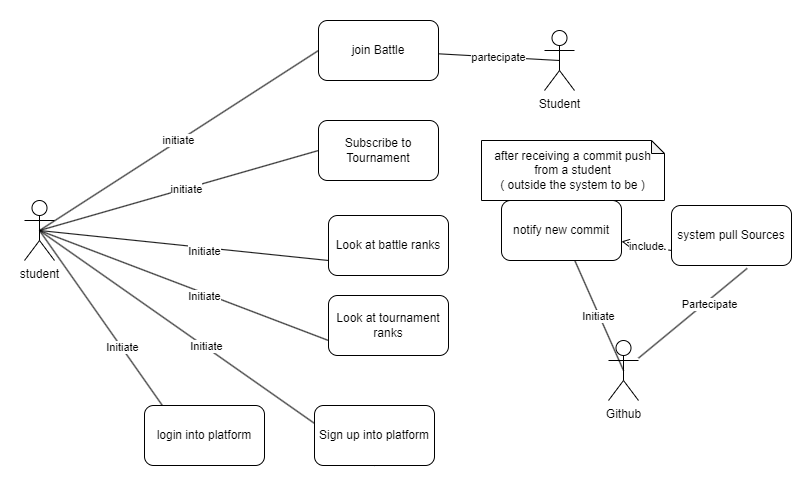
\includegraphics[width=1\linewidth]{misc//Images//UC/StudentScenarios.png}
    \caption{Student Use Case Diagram}
    \label{fig:enter-label}
\end{figure}


\subsubsection{Educator Use Case Diagram}
\begin{figure}[H]
    \centering
    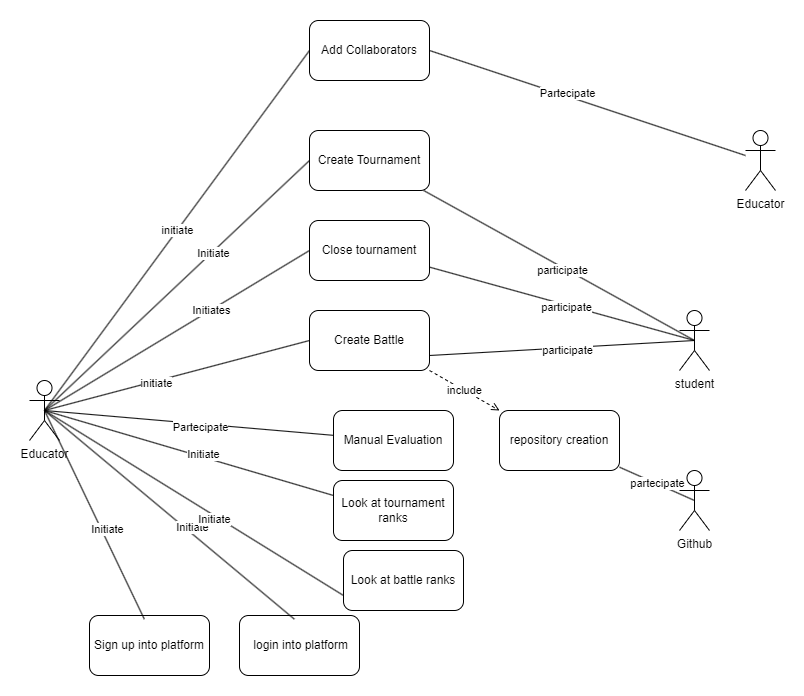
\includegraphics[width=1\linewidth]{misc//Images//UC/EducatorScenarios.png}
    \caption{Educator Use Case Diagram}
    \label{fig:enter-label}
\end{figure}

\subsection{Use Cases}
In this section we analyze the various use cases of the system by describing the actors, entry conditions, event flow, exit conditions and exceptions for all of them.

\newpage
\subsubsection{UC1: Sign Into Platform}
\begin{center}
    \begin{longtable}{lp{0.75\linewidth}}
        \hline
            Actor & Users(Educators, Students)\\
        \hline
            Entry condition & A user accesses the platform for the very first time\\
        \hline
            Event Flow & 1. User reaches the platform\\
                &2. User clicks on "sign in" button\\
                &3. User fills out own info and decides if they want to be an Educator or student\\
                &4. User concludes the registration by clicking "finish" button\\
        \hline
            Exit & User is successfully registered on the platform as either educator or student\\
        \hline
            Exception & Missing or wrong input by user during registration form\\
        \hline
    \end{longtable}
\end{center}


\begin{figure}[H]
    \centering
    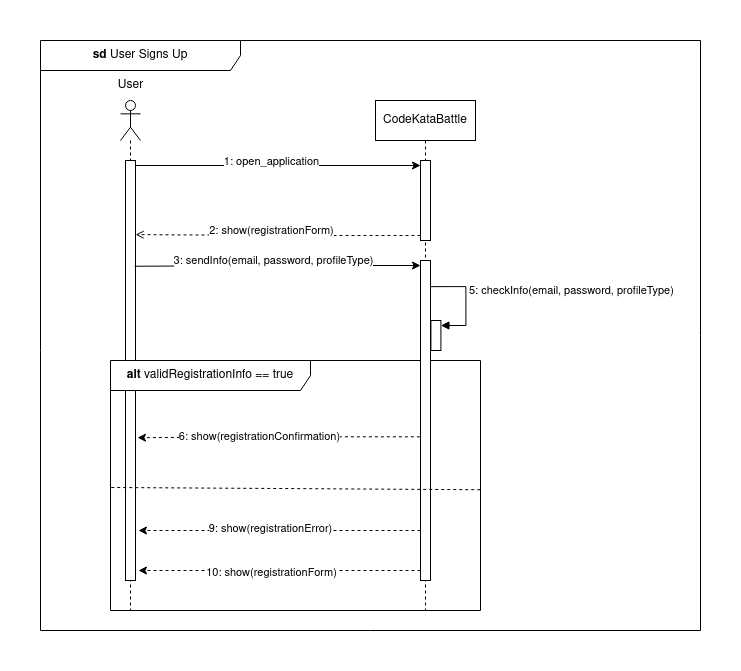
\includegraphics[width=1\linewidth]{misc//Images//UC Diagrams/UC1.png}
    \caption{User Signs Up sequence diagram}
    \label{fig:enter-label}
\end{figure}

\subsubsection{UC2: Log Into Platform}
\begin{center}
    \begin{longtable}{lp{0.75\linewidth}}
        \hline
            Actor & User\\
        \hline
            Entry condition & User is signed into platform\\
        \hline
            Event Flow & 1. User reaches the platform\\
                       & 2. User clicks on "log in" button\\
                       & 3. User fills out email and password used during registration\\
                       & 4. User completes login by clicking "confirm" button\\
        \hline
            Exit & User is successfully logged into platform\\
        \hline
            Exception & Missing or wrong input by user during log in form\\
        \hline
    \end{longtable}
\end{center}

\begin{figure}[H]
    \centering
    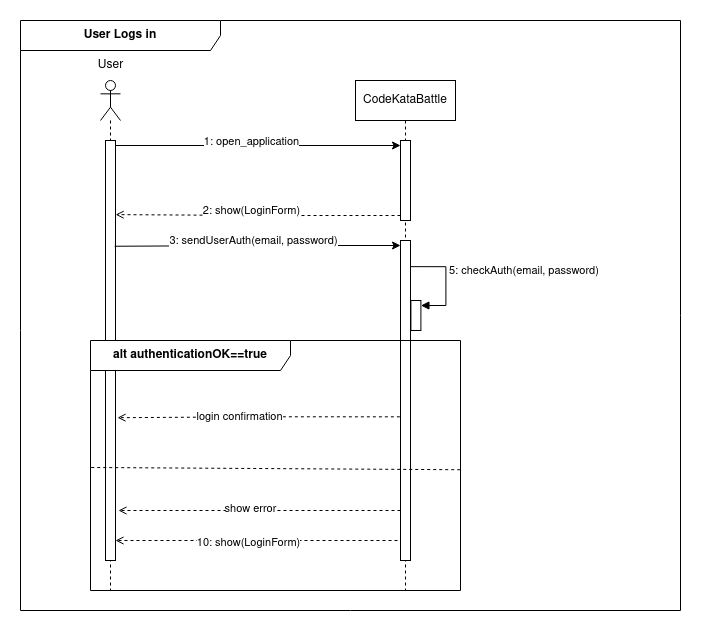
\includegraphics[width=1\linewidth]{misc//Images//UC Diagrams/UC2.png}
    \caption{Create tournament sequence diagram}
    \label{fig:enter-label}
\end{figure}

\newpage
\subsubsection{UC3: Create Tournament}
\begin{center}
    \begin{longtable}{lp{0.75\linewidth}}
        \hline
            Actor & Educator, Students\\
        \hline
            Entry condition & Educator is logged into the platform\\
        \hline
            Event Flow &  1. Educator presses "Create Tournament" button\\
                       &  2. Educator fills out details of tournament\\
                       &  3. Educator adds other collaborators to tournament(other Educators)\\
                       &  4. Educator completes tournament creation\\
                       &  5. Platform notifies all Students of new tournament\\
        \hline
            Exit & Tournament is created successfully \\
        \hline
            Exception & Missing or wrong input by Educator during tournament creation form\\
        \hline
    \end{longtable}
\end{center}

\begin{figure}[H]
    \centering
    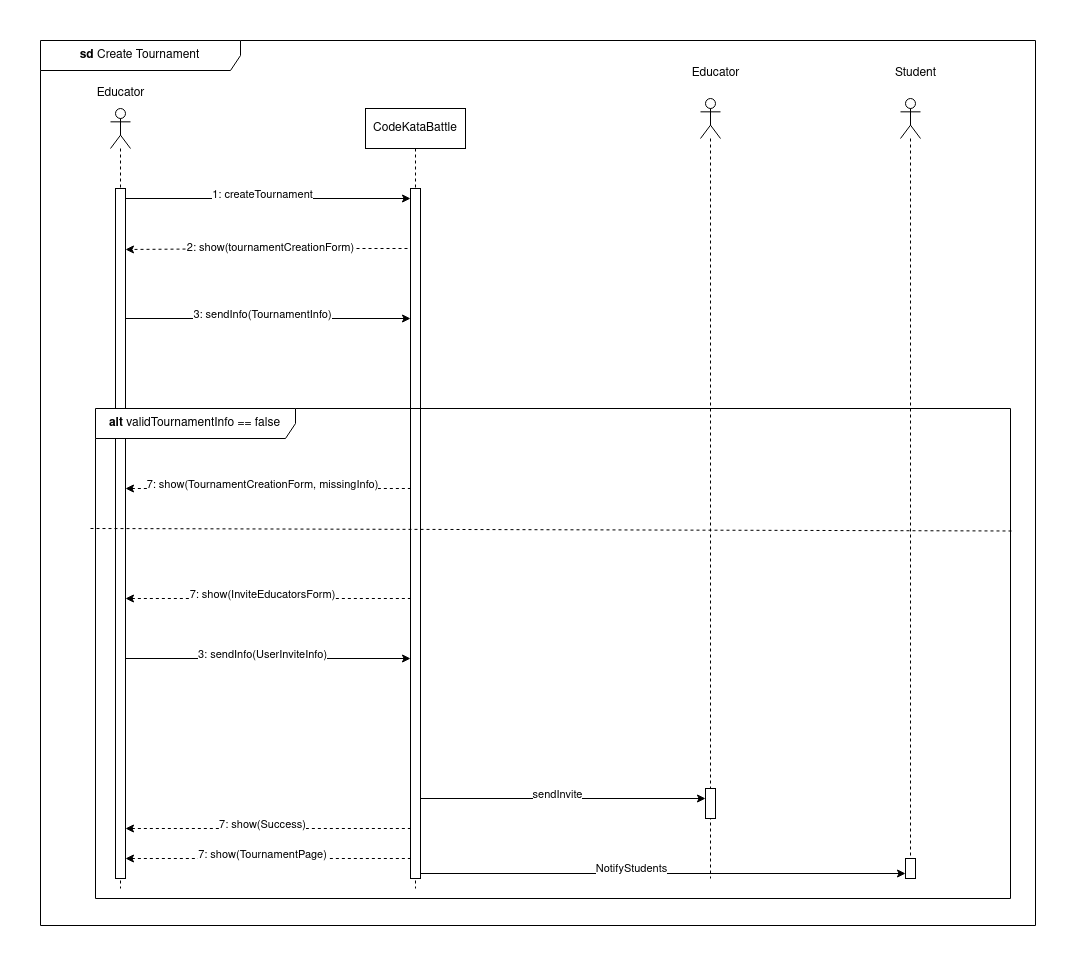
\includegraphics[width=1\linewidth]{misc//Images//UC Diagrams/UC3.png}
    \caption{Create tournament sequence diagram}
    \label{fig:enter-label}
\end{figure}

\newpage
\subsubsection{UC4: Subscribe to Tournament}
\begin{center}
    \begin{longtable}{lp{0.75\linewidth}}
        \hline
            Actor & Students\\
        \hline
            Entry condition & Student is logged into the platform\\
        \hline
            Event Flow & 1. Student is notified of new tournament\\
                       & 2. Student presses "Join tournament" button\\
        \hline
            Exit & Student is subscribed to tournament\\
        \hline
            Exception & \\
        \hline
    \end{longtable}
\end{center}

\begin{figure}[H]
    \centering
    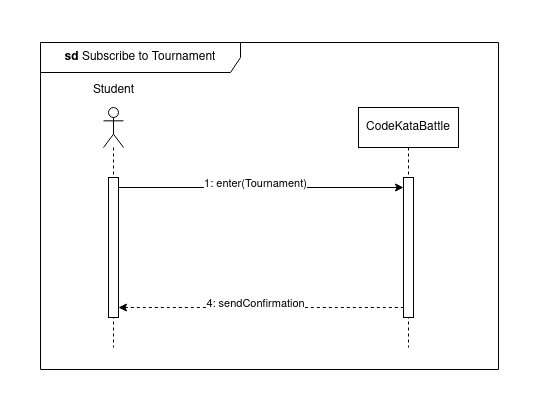
\includegraphics[width=1\linewidth]{misc//Images//UC Diagrams/UC4.png}
    \caption{Subscribe to Tournament sequence diagram}
    \label{fig:enter-label}
\end{figure}

\newpage
\subsubsection{UC5: Create Battle}
\begin{center}
    \begin{longtable}{lp{0.75\linewidth}}
        \hline
            Actor & Educator, Student\\
        \hline
            Entry condition & Educator has logged in and is inside the context of a tournament\\
        \hline
            Event Flow & 1. Educator press "create new battle" button\\
                       & 2. Educator upload the \ac{CK} assignment, tests and project build\\
                       & 3. Educator sets subscription and submission deadlines and group size rules\\
                       & 4. Educator complete battle creation\\
                       & 5. The platform sends notification to all the students subscribed to the tournament\\
        \hline
            Exit & Battle created correctly\\
        \hline
            Exception & Missing or wrong input by Educator\\
        \hline
    \end{longtable}
\end{center}

\begin{figure}[H]
    \centering
    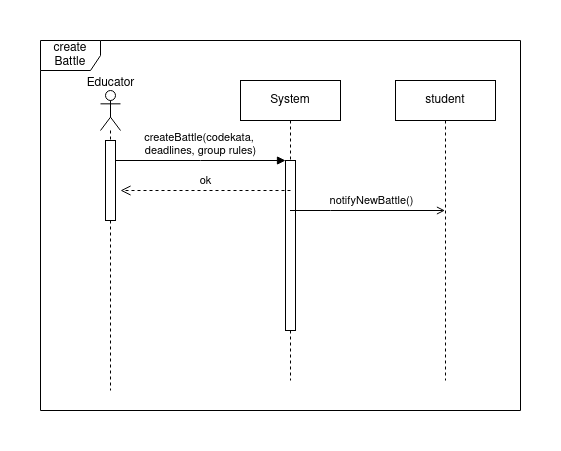
\includegraphics[width=1\linewidth]{misc//Images//UC Diagrams/UC5.png}
    \caption{Create Battle sequence diagram}
    \label{fig:enter-label}
\end{figure}

\newpage
\subsubsection{UC6: Join Battle}
\begin{center}
    \begin{longtable}{lp{0.75\linewidth}}
        \hline
            Actor & Student\\
        \hline
            Entry condition & Student subscribed to a tournament, student logged in, battle available for subscription in tournament\\
        \hline
            Event Flow  & 1. Student press "join battle" button in tournament context\\
                        & 2. platform shows group size rules\\
                        & 3. student uses "invite" button\\
                        & 4. Student inserts other students identifiers\\
                        & 5. other students accepts invite\\
                        & 6. Group of student is created\\
                        & 7. Group of students joins battle\\
        \hline
            Exit & Student group joins battle\\
        \hline
            Exception & \\
        \hline
    \end{longtable}
\end{center}

\begin{figure}[H]
    \centering
    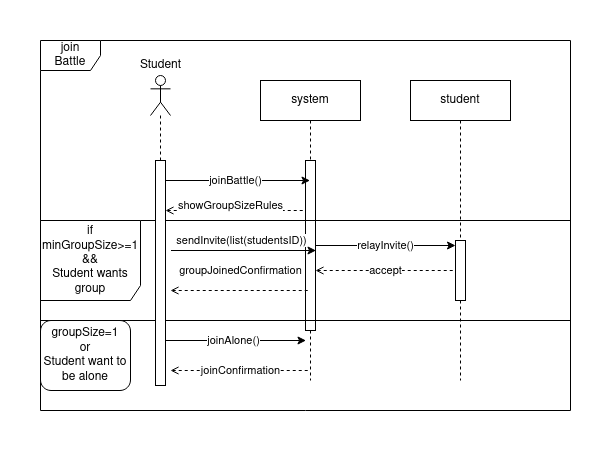
\includegraphics[width=1\linewidth]{misc//Images//UC Diagrams/UC6.png}
    \caption{Join Battle sequence diagram}
    \label{fig:enter-label}
\end{figure}

\newpage
\subsubsection{UC7: Create Repository}
\begin{center}
    \begin{longtable}{lp{0.75\linewidth}}
        \hline
            Actor & Github, Student\\
        \hline
            Entry condition & Subscription deadline of battle expired\\
        \hline
            Event Flow & 1. The platform creates a repository for the codekata battle in github\\
                       & 2. The platform sends to all students subscribed to the battle the link to the repository\\
        \hline
            Exit & Student recieve repository link\\
        \hline
            Exception & \\
        \hline
    \end{longtable}
\end{center}

\begin{figure}[H]
    \centering
    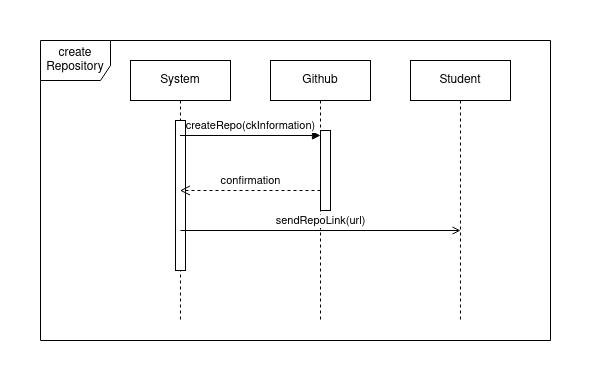
\includegraphics[width=1\linewidth]{misc//Images//UC Diagrams/UC7.png}
    \caption{Create Repository sequence diagram}
    \label{fig:enter-label}
\end{figure}

\newpage
\subsubsection{UC8: Score Commit}
\begin{center}
    \begin{longtable}{lp{0.75\linewidth}}
        \hline
            Actor & GitHub\\
        \hline
            Entry condition & Github notified platform of student commit\\
        \hline
            Event Flow & 1. Platform receives notification of commit\\
                       & 2. Platform pulls sources and compiles them\\
                       & 3. Platform starts evaluation(functional, timeliness, quality)\\
                       & 4. Platform updates score for battle\\
        \hline
            Exit & Battle leader board is updated\\
        \hline
            Exception & Compilation of sources fails\\
        \hline
    \end{longtable}
\end{center}

\begin{figure}[H]
    \centering
    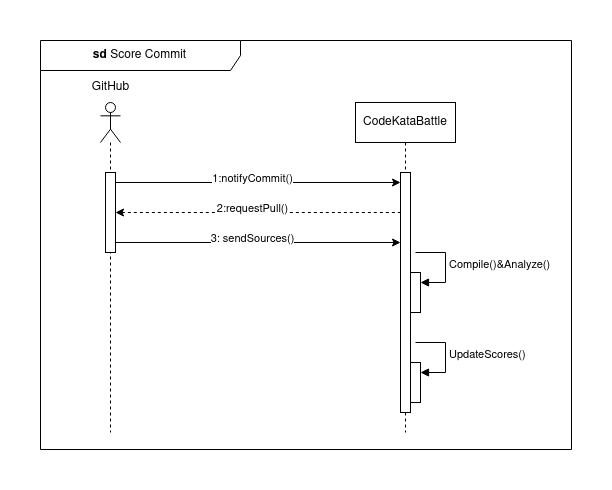
\includegraphics[width=1\linewidth]{misc//Images//UC Diagrams/UC8.png}
    \caption{Score Commit sequence diagram}
    \label{fig:enter-label}
\end{figure}

\newpage
\subsubsection{UC9: View Battle Ranking}
\begin{center}
    \begin{longtable}{lp{0.75\linewidth}}
        \hline
            Actor & User(Educators, Students)\\
        \hline
            Entry condition & Educator is involved with tournament of the battle, student has joined battle\\
        \hline
            Event Flow & 1. User press "view ranking" button in battle context\\
                       & 2.platform shows ranking table\\
        \hline
            Exit & User sees ranking table\\
        \hline
            Exception & \\
        \hline
    \end{longtable}
\end{center}

\begin{figure}[H]
    \centering
    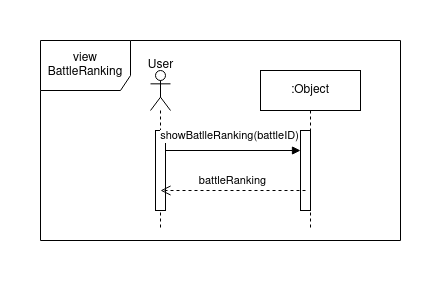
\includegraphics[width=1\linewidth]{misc//Images//UC Diagrams/UC9.png}
    \caption{View Battle Ranking sequence diagram}
    \label{fig:enter-label}
\end{figure}

\newpage
\subsubsection{UC10: Manual Evaluation}
\begin{center}
    \begin{longtable}{lp{0.75\linewidth}}
        \hline
            Actor & Educators\\
        \hline
            Entry condition & Battle deadline Expires\\
        \hline
            Event Flow & 1. Platform notifies educators that battle ha ended and manual evaluation is required(as decided during battle creation)\\
                       & 2. Educators use platform to analyze sources\\
        \hline
            Exit & Educator add a manual score\\
        \hline
            Exception & Educator adds illegal score\\
        \hline
    \end{longtable}
\end{center}

\begin{figure}[H]
    \centering
    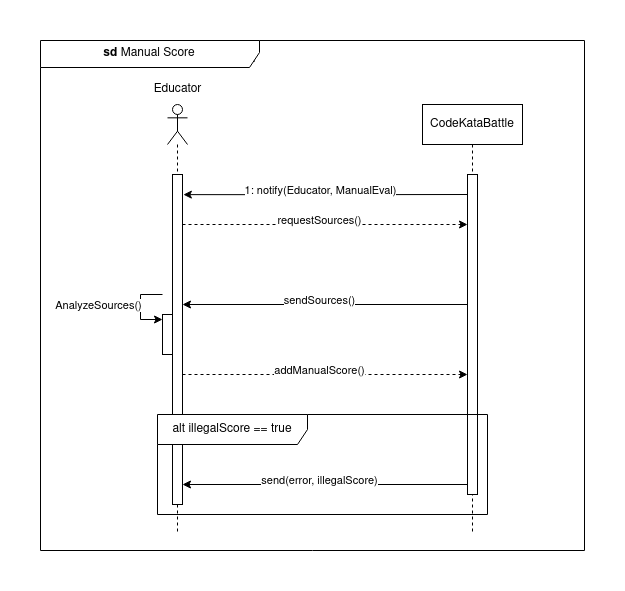
\includegraphics[width=1\linewidth]{misc//Images//UC Diagrams/UC10.png}
    \caption{Manual Evaluation sequence diagram}
    \label{fig:enter-label}
\end{figure}

\newpage
\subsubsection{UC11: Look at tournament ranks}
\begin{center}
    \begin{longtable}{lp{0.75\linewidth}}
        \hline
            Actor & Students, Educators\\
        \hline
            Entry condition & Student or Educator are on the main tournament page and are involved\\
        \hline
            Event Flow & 	Student or educator click on tournament leader-board\\
        \hline
            Exit & 	Platform shows Tournament leader board\\
        \hline
            Exception & Tournament hasn't yet started \\
        \hline
    \end{longtable}
\end{center}

\begin{figure}[H]
    \centering
    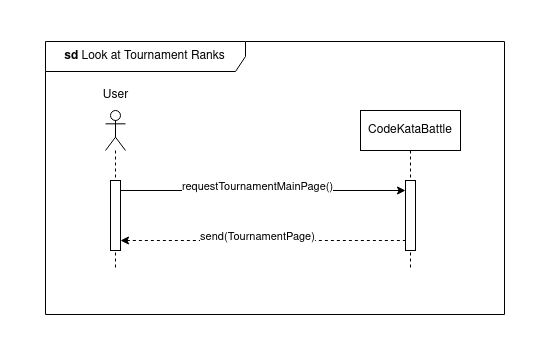
\includegraphics[width=1\linewidth]{misc//Images//UC Diagrams/UC11.png}
    \caption{Look at tournament ranks sequence diagram}
    \label{fig:enter-label}
\end{figure}

\newpage
\subsubsection{UC12: Close Tournament}
\begin{center}
    \begin{longtable}{lp{0.75\linewidth}}
        \hline
            Actor & Educator, Student\\
        \hline
            Entry condition & Educator logged in, Tournament still ongoing, no ongoing battle\\
        \hline
            Event Flow & 1. Edu press "close tournament" in the tournament context\\
& 2. The platform closes the tournament\\
& 3. The platform notifies all the students subscribed to the tournament\\
        \hline
            Exit & Tournament closed, platform notifies students\\
        \hline
            Exception & \\
        \hline
    \end{longtable}
\end{center}

\begin{figure}[H]
    \centering
    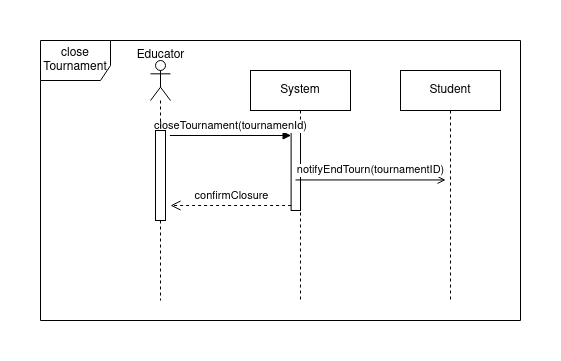
\includegraphics[width=1\linewidth]{misc//Images//UC Diagrams/UC12.png}
    \caption{Close Tournament sequence diagram}
    \label{fig:enter-label}
\end{figure}


\newpage
\subsection{Mapping on requirements}

\begin{center}
    \begin{longtable}{l p{0.75\linewidth}}
        \hline
            \textbf{Use Case} & \textbf{Requirements}\\
        \hline
            UC1 & R10\\
        \hline
            UC2 & R5, R6\\
        \hline
            UC3 & R6, R2.1, R1, R14\\
        \hline
            UC4 & R5, R3\\
        \hline
            UC5 & R6, R2, R2.1, R2.2, R2.3, R2.4, R2.5, R15\\
        \hline
            UC6 & R5, R4, R4.1, R15\\
        \hline
            UC7 & R18, R19\\
        \hline
            UC8 & R9, R9.1, R13, R13.1\\
        \hline
            UC9 & R5, R6, R13, R13.1\\
        \hline
            UC10 & R6, R7, R2.5, R16\\
        \hline
            UC11 & R5, R6, R8, R8.1\\
        \hline
            UC12 & R6, R17, R11\\
        \hline
        
    \end{longtable}
\end{center}

\section{Design Constraints}
\subsection{Standards compliance}
First of all, the system should respect all the laws regarding privacy and data treatment and exchange with third parties (i.e. CPOs); to work in Europe, the system should respect the EU GDPR. In particular, a general description of the main principles that data should have in order to guarantee their privacy is given in Art. 5 of the GDPR document.

\subsection{Hardware limitations}
There are no hardware contraints.

\subsection{Any other constraint}
There are no other constraints.

\section{Software System Attributes}
\subsection{Reliability}
The system should be able to restart automaticly shortly after an interruption and recover the previous backupped state.

\subsection{Availability}
The system should be operative at least 99\% of the time to avoid the impairment of activities with deadlines and in case of downtime the system should recover any missed notification received from GitHub on group commit in battles when it restarts.

\subsection{Security}
The system should ensure safety of the user credentials and it should keep log of access and of sensible operations, such as in the case of educator closing a tournament or manually evaluation of sources, to avoid malicious use of the educator authority.

\subsection{Maintainability}
The development should follow good practice for maintainability, such as dividing the system in enough modules depending on the functionalities. This is necessary in order to facilitate maintenance and substitution of modules. Every functionality needs to be well documented.

\subsection{Portability}
The platform as a website should behave as expected on at least the most used browsers, without requiring additional effort from the end user. The back end should be written in a language that ensures portability and its functionalities should not be reliant on a particular compiler of system.

\newpage

\chapter{Formal analysis using Alloy}
\section{Alloy Code}

\begin{lstlisting}[language=alloy,label={lst:alloy_code}]
open util/integer

abstract sig User{}

sig Educator extends User{
	tournamentsInvolved : set Tournament
}

sig Student extends User{
	tournamentRank : disj set RankTournament,
	subscribedTournaments : set Tournament,
}

sig Group{
	students : some Student,
	battleRank: disj one RankBattle 
}{this in Battle.currentGroups}

sig Tournament{
	battleList : disj some Battle,
	leaderBoard : disj one LeaderboardTournament
}{this in Educator.tournamentsInvolved }

sig Battle{
	currentGroups : disj set Group,
	assignment : disj one CodeKata,
	rules :disj one Rules,
	repo : disj lone Repository,
	leaderBoard: disj one LeaderboardBattle ,
    battleStatus : one BattleStatus
}{this in Tournament.battleList}

sig LeaderboardBattle{
	positions : disj set RankBattle
}{this in Battle.leaderBoard}

sig LeaderboardTournament{
	positions : disj set RankTournament
}{this in Tournament.leaderBoard}

sig RankTournament extends Rank{
    studentScore : disj one StudentScore
}{this in LeaderboardTournament.positions and this in Student.tournamentRank }

sig RankBattle extends Rank{
    battleScore : disj lone GroupScore
}{this in LeaderboardBattle.positions and this in Group.battleRank}

sig Repository{}{this in Battle.repo}

sig CodeKata{
	testCases : disj one TestCase
}{this in Battle.assignment}

sig TestCase{}{this in CodeKata.testCases}

sig Rules{
	minSize : Int,
	maxSize : Int,
	subscriptionDeadline :one DateTime,
	submissionDeadline:one DateTime
}{this in Battle.rules}

abstract sig Score{}
sig StudentScore extends Score{}{this in RankTournament.studentScore}
sig GroupScore extends Score{}{this in RankBattle.battleScore}

abstract sig Rank{
}

sig DateTime{}{this in Rules.submissionDeadline and this in Rules.subscriptionDeadline}

abstract sig TournamentStatus{}
one sig OpenTournament extends TournamentStatus{}
one sig ClosedTournament extends TournamentStatus{}

abstract sig BattleStatus{}
one sig SubscriptionOpen extends BattleStatus{} //no ranking no repo in battle, 
one sig SubmissionOpen extends BattleStatus{} 
one sig ConsolidationPhase extends BattleStatus{}
one sig BattleClosed extends BattleStatus{} // 

///---------------------------------------------FACTS---------------------------------------

fact noRepoInSubscriptionPhase{
    all b : Battle | b.battleStatus=SubscriptionOpen iff (no b.repo)
}

fact minLessThanMaxSize{
	all r :Rules | (int r.minSize>=1 and int r.minSize<=int r.maxSize) 
}
fact respectSizeRule{
	all b : Battle | 
		(all g : Group | 
			(g in b.currentGroups implies ( int #g.students>=int b.rules.minSize and int #g.students<=int b.rules.maxSize) )
		)
}

fact studentInOneGroupForBattle{
	all battle : Battle | (
		all disj g1,g2 : Group |( g1 in battle.currentGroups and g2 in battle.currentGroups implies (
			no s : Student | s in g1.students and s in g2.students)
		) 
	)
}

fact rankAssociatedToBattleLeaderboard{
	all b : Battle | (
		all g : Group | g in b.currentGroups iff (g.battleRank in b.leaderBoard.positions)
	)
}
fact oneRankForTournament{//this implies that for every tournament the student is in there is only one rank and for every rank there is only one tournament subscribed
	all s: Student |(all t : Tournament | t in s.subscribedTournaments implies one r: Rank| r in s.tournamentRank and r in t.leaderBoard.positions)
					and (all r :RankTournament | r in s.tournamentRank implies (one t : Tournament| t in s.subscribedTournaments and r in t.leaderBoard.positions))
	
//without the 2 predicates there could be case were a student had 2 ranks for a tournament he wasnt in
}

fact ifInBattleThenInTournament{
	all t : Tournament | (
		all b : Battle | (
			all g : Group | (
				all st: Student | (g in b.currentGroups and st in g.students and b in t.battleList) implies t in st.subscribedTournaments
			)
		)
	)
}
 
fact mustBeGroupsInStartedBattle{
	all b :Battle| b.battleStatus!=SubscriptionOpen implies some g:Group |g in b.currentGroups

}

///---------------------------------------------------PREDICATES--------------------------------


pred noWrongRankLogic{//to test no student can have a score and rank within a tournament without being subscribed to said tournament
	(some s:Student| (some t: Tournament | t in s.subscribedTournaments and no r:Rank| r in s.tournamentRank) )
}

pred noStudentInTwoGroupBattle{//to test no student can join 2 groups for a battle
	some b : Battle| (some disj g1, g2 :Group| g1 in b.currentGroups and g2 in b.currentGroups and (	one s: Student | s in g1.students and s in g2.students) 
	)
}


pred show{}

pred showGenericTournaments{
	some Tournament
	#Battle>1
}


pred showSomeRealistic{
	#Student > 4
	#Tournament > 1
	#Group > 1
	#Battle.currentGroups > 0
	Rules.maxSize<5
	one s : Student| no g:Group| s in g.students 
}


pred showNoGroupBattle{//effectiviely a battle can have no subscribed groups only if it is within the subscription deadline
	one Battle 
	lone s:Student |  #s.subscribedTournaments>0
	no Group
}
pred joinNewBattle[s : Student]{//shows an instance where a student "s" joined with 2 other student a battle as a group
	one b : Battle| b.battleStatus=SubscriptionOpen and (one g:Group| s in g.students and g in b.currentGroups and  #g.students=3)

}
pred joinTournament[s:Student]{//shows a student joining an existing tournament 
	one t:Tournament| t in s.subscribedTournaments
	one Tournament
	one Student

}
run joinTournament for 6
\end{lstlisting}


\section{Simulations}
In this section we show some of the simulations of the built model.


\begin{sidewaysfigure}
    \begin{figure} [H]
        \begin{center}
            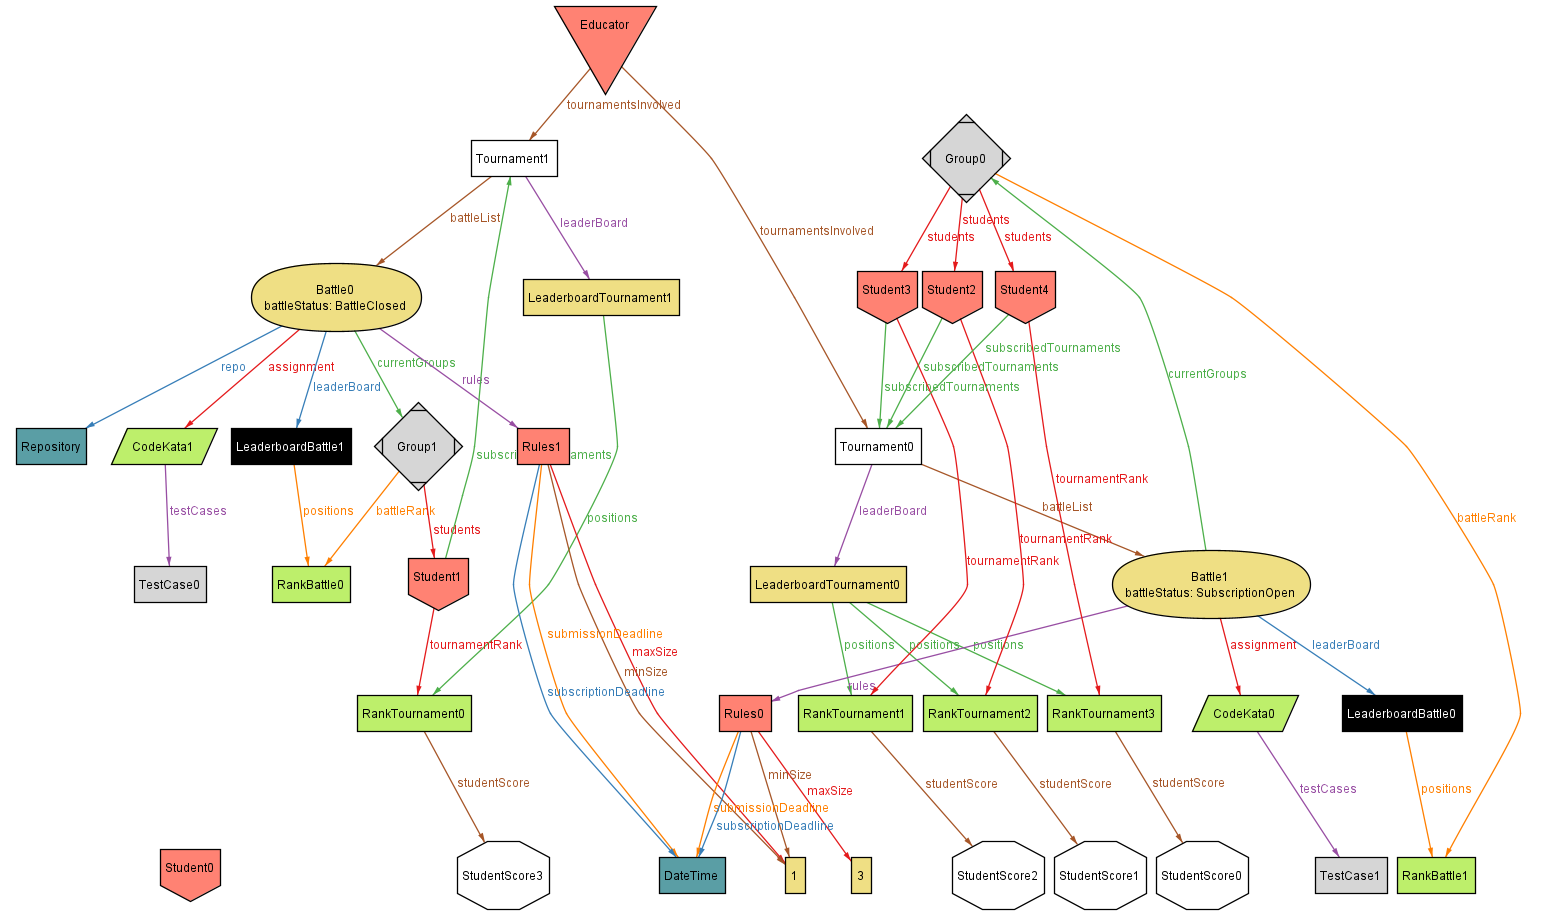
\includegraphics[width=1\linewidth]{misc/Images/AlloySims/showSomeRealistic.png}
            \caption{Simple world Alloy.}
        \end{center}
    \end{figure}
\end{sidewaysfigure}


\begin{figure}
    \centering
    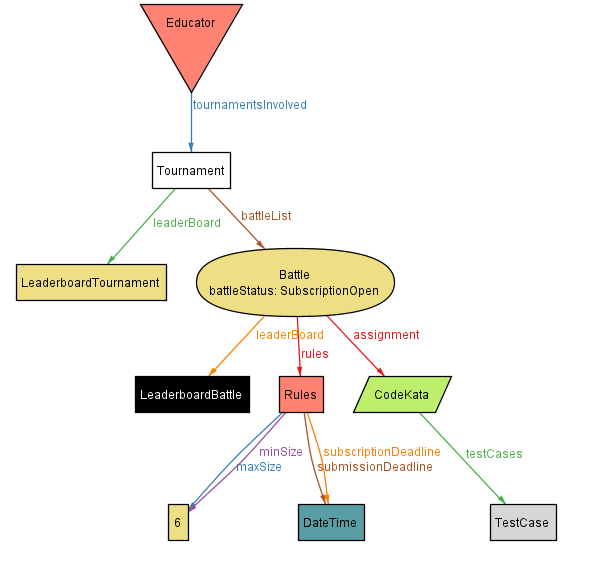
\includegraphics[width=1\linewidth]{misc//Images//AlloySims/noGroupBattle.png}
    \caption{Battle with no groups}
\end{figure}

\begin{figure}[!]
    \centering        
            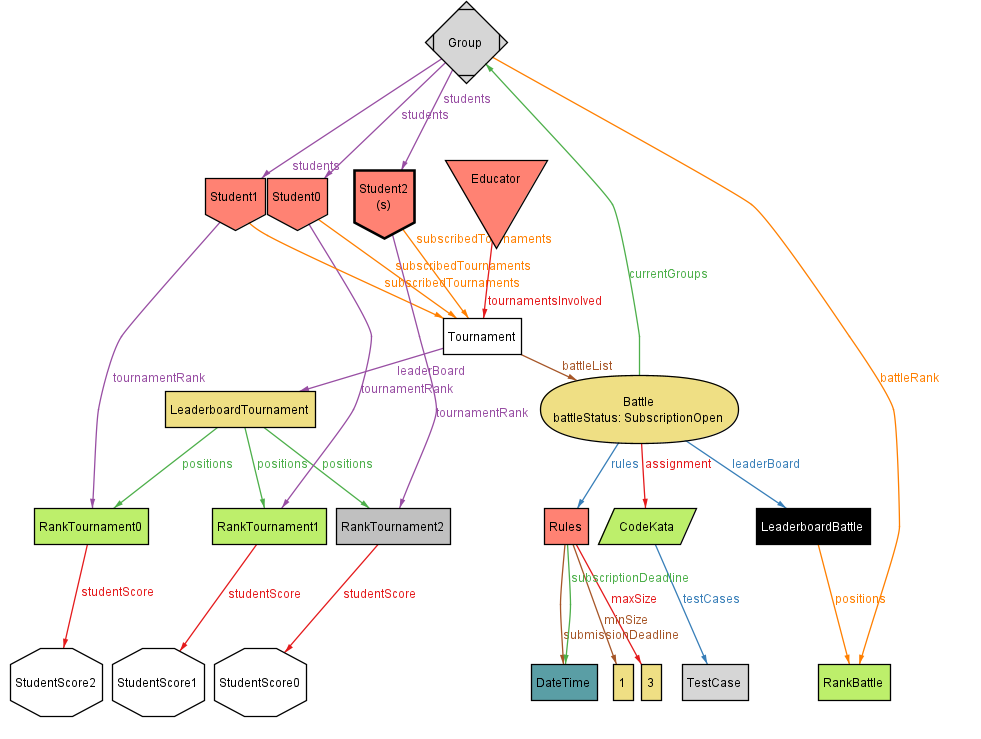
\includegraphics[width=1.3\linewidth]{misc//Images//AlloySims/joinNewBattle.png}
            \caption{Student joins a battle with a group}    
    
\end{figure}


\begin{figure}
    \centering
    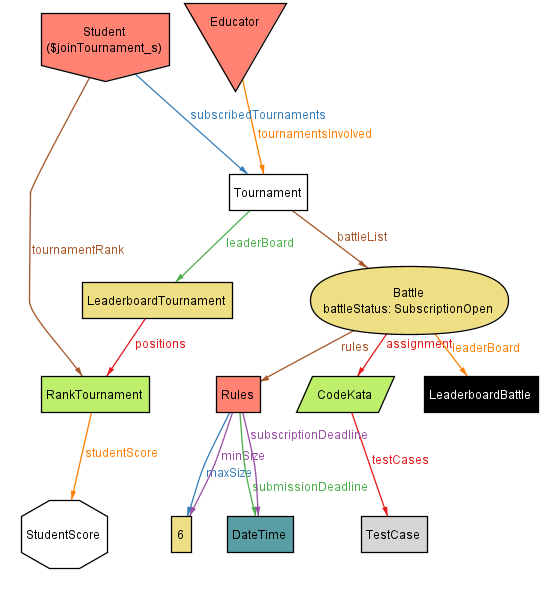
\includegraphics[width=1\linewidth]{misc//Images//AlloySims/joinTournament.png}
    \caption{Student joins a tournament}
    \label{fig:enter-label}
\end{figure}


%HERE IMAGES OF SIMULATIONS
\newpage

\chapter{Effort spent}

\begin{table}[h]
    \centering
    \scalebox{1.5}{
    \begin{tabular}{|c | c | c|}
    \hline
        \textbf{Chapter} & \textbf{Valentino} & \textbf{Zarbo} \\ \hline
        1 & 3 & 2\\ \hline
        2 & 16 & 20\\ \hline
        3 & 3 & 5\\ \hline
        4 & 7 & 2 \\ \hline
        5 & 4 & 4\\ \hline
    \end{tabular}
    }
    \caption{Time Spent in hours for each chapter}
    \label{tab:my_label}
\end{table}


\newpage

\chapter{References}
\section{Used tools}
\begin{itemize}
    \item \href{https://github.com/}{GitHub} for project versioning
    \item \href{https://www.overleaf.com}{Overleaf} as \LaTeX\ editor
    \item \href{https://www.jetbrains.com/idea/}{IntelliJ Idea} as Java IDE
\end{itemize}

\end{document}
